%********************************************************************
% Appendix
%*******************************************************
% If problems with the headers: get headings in appendix etc. right
\markboth{\spacedlowsmallcaps{Appendix}}{\spacedlowsmallcaps{Appendix}}
%************************************************
\chapter{Appendix A: VESC Board Schematic Files}\label{appendix:vesc_schematics}

\begin{sidewaysfigure}[ht]
    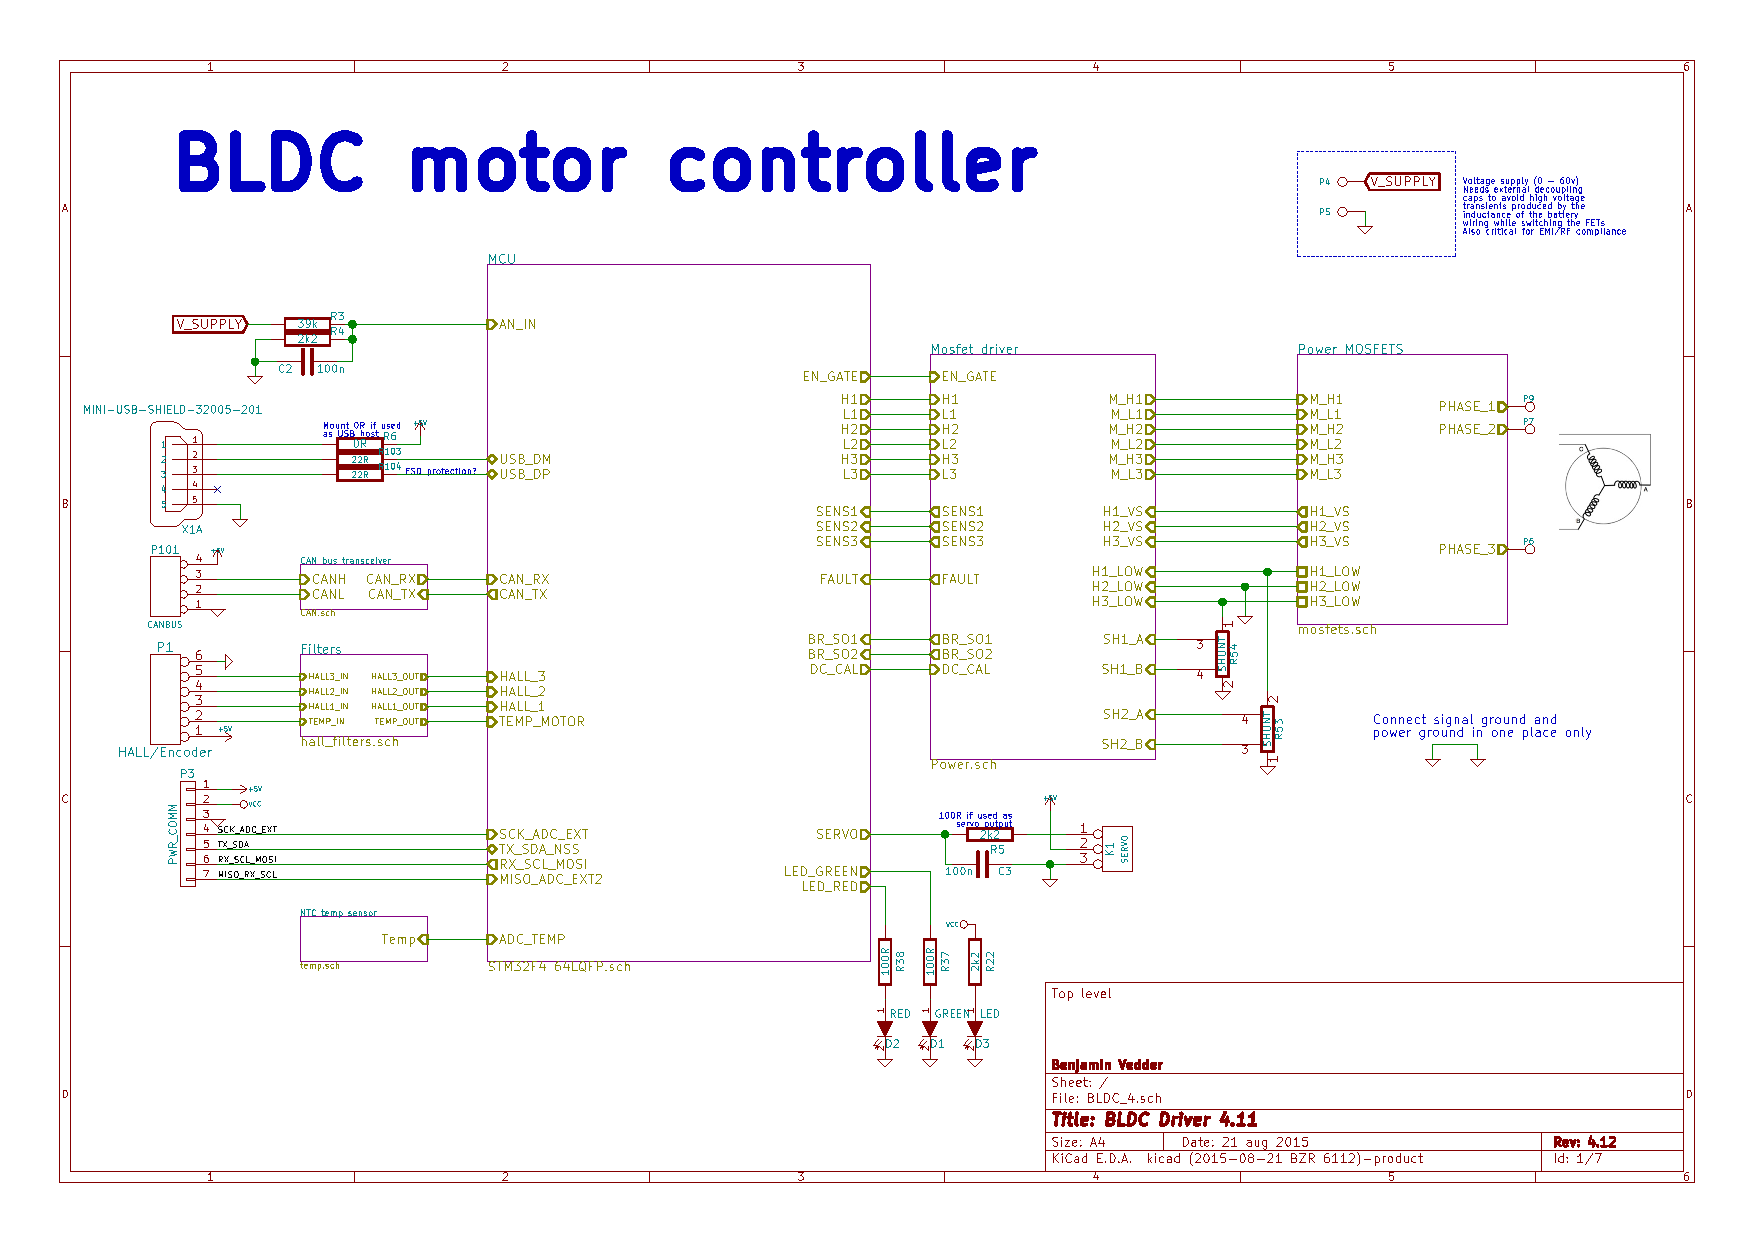
\includegraphics[width=\textwidth,page=1]{Images/BLDC_4}
    \caption{Schematic Overview}
    \label{fig:sch1}
\end{sidewaysfigure}

\begin{sidewaysfigure}[ht]
    \includegraphics[width=\textwidth,page=2]{Images/BLDC_4}
    \caption{Three-Phase MOSFET Inverter}
    \label{fig:sch2}
\end{sidewaysfigure}

\begin{sidewaysfigure}[ht]
    \includegraphics[width=\textwidth,page=3]{Images/BLDC_4}
    \caption{In-Board Temperature Sensor}
    \label{fig:sch3}
\end{sidewaysfigure}

\begin{sidewaysfigure}[ht]
    \includegraphics[width=\textwidth,page=4]{Images/BLDC_4}
    \caption{CAN Bus Transceiver}
    \label{fig:sch4}
\end{sidewaysfigure}

\begin{sidewaysfigure}[ht]
    \includegraphics[width=\textwidth,page=5]{Images/BLDC_4}
    \caption{Hall Effect Sensors Signal Conditioning}
    \label{fig:sch5}
\end{sidewaysfigure}

\begin{sidewaysfigure}[ht]
    \includegraphics[width=\textwidth,page=6]{Images/BLDC_4}
    \caption{STM32F405 Hardware Setup}
    \label{fig:sch6}
\end{sidewaysfigure}

\begin{sidewaysfigure}[ht]
    \includegraphics[width=\textwidth,page=7]{Images/BLDC_4}
    \caption{DRV8302 MOSFET Driver}
    \label{fig:sch7}
\end{sidewaysfigure}

%\section{The \texttt{listings} package to include source code}
%Source code is usually not part of the text of a thesis, but if it is an original contribution it makes sense to le the code speak by itself instead of describing it. The package \verb!listings! provide the proper layout tools. Refer to its manual if you need to use it, an example is given in listing \ref{lst:probCounter}.